\documentclass[a4paper, 12pt]{article}
\usepackage[T2A,T1]{fontenc}
\usepackage[utf8]{inputenc}
\usepackage[english, russian]{babel}
\usepackage{graphicx}
\graphicspath{{img/}}
\usepackage[hcentering, bindingoffset = 10mm, right = 15 mm, left = 15 mm, top=20mm, bottom = 20 mm]{geometry}
\usepackage{amsmath, amstext}
\usepackage{float}
\usepackage{wasysym}
\setlength{\parindent}{0em}
\setlength{\parskip}{0.5em}
\renewcommand{\arraystretch}{1.2}

\newenvironment{bottompar}{\par\vspace*{\fill}}{\clearpage}
 
\begin{document}

\begin{titlepage}
\newcommand{\HRule}{\rule{\linewidth}{0.5mm}} % Defines a new command for the horizontal lines, change thickness here

\center % Center everything on the page
 
\textsc{\LARGE Московский\\[-0.2cm]Физико-Технический Институт\\[0.1cm]\large (государственный университет)}\\[1.5cm] % Name of your university/college
\textsc{\Large Кафедра общей физики}\\[0.1cm] % Major heading such as course name
\textsc{\large Вопрос по выбору, ГКЭ}\\[0.5cm] % Minor heading such as course title

\HRule
\\[0.8cm]
{ \huge \bfseries Фазовые переходы второго рода\\[0.3cm]  и их механическая аналогия}
\\[0.8cm] % Title of your document
\HRule
\\[1.5cm]

\begin{flushleft} \large
	\textsf{Студент}\\[0.1cm]
	Ушаков Роман \\
	511 группа
\end{flushleft}

\begin{bottompar}
	\begin{center}
		
\includegraphics[width = 80 mm]{logo.jpg}
	\end{center}
	{\large \today}

\end{bottompar}
\vfill
\end{titlepage}


\subsection*{Теория}

\emph{Фаза} ~--- макроскопическая физически однородная часть вещества, отделённая от остальных частей границами раздела, так что она может быть извлеченая из системы механическим путём.

Рассмотрим систему, которая состоит из двух фаз 1 и 2, которые могут превращаться друг в друга. Для механического и теплового равновесия необходимо, чтобы $T_1 = T_2$ и $P_1 = P_2$. Пусть $m_1$ и $m_2$ соответственно массы фаз, а $\varphi_1$ и $\varphi_2$  ~--- удельные термодинамические потенциалы вещества в этих фазах. Тогда очевидно, что термодинамический потенциал всей системы $\Phi = m_1 \varphi_1 + m_2 \varphi_2$. Напомним, что термодинамический потенциал системы по определению равен $\Phi = \Phi(P, T) = U - TS + PV$, поэтому если при фазовых превращениях $T = ~const$ и $P =~const$, то $\varphi_1$ и $\varphi_2$ не будут меняться. Следовательно, при фазовых превращениях меняются только массы $m_1$ и $m_2$, и эти превращения должны происходить в таком направлении, чтобы $\Phi$ принял наименьшее значение, которое возможно в рассматриваемых условиях. Поэтому только при условии $\varphi_1(P, T) = \varphi_2(P, T)$ фазы будут находиться в равновесии друг с другом.

Мы получили следующее важное следствие: при всех изменениях состояния вещества его удельный термодинамический потенциал всегда меняется непрерывно (в отличии от других величин ~--- удельного объема, удельной энтропии и пр.).

Фазовые превращения, при которых первые производные функции $\varphi(P, T)$ меняются скачкообразно, называются \emph{фазовыми превращениями первого рода}. Фазовые превращения, в которых первые производные остаются непрерывными, а вторые производные меняются скачкообразно, называются \emph{фазовыми переходами второго рода}.

Так как $ d \varphi = - s dT + v d P$, то:
$$
	s = - \left( \frac{\partial \varphi }{\partial T} \right)_{P} \text{ и } 
	v = \left( \frac{\partial \varphi }{\partial P} \right)_{T} 
$$

Следовательно, фазовые переходы первого рода характеризуются скачкообразным изменением либо удельной энтропии $s$, либо удельного объема $v$, либо обеих величин сразу. Скачкообразное изменение энтропии означает выделение или поглощение тепла. Следовательно, фазовые переходы второго рода не сопровождаются выделением или поглощением теплоты, а также изменением удельного объема вещества. Таким образом, фазовый переход второго рода является непрерывным в том смысле, что состояние тела меняется непрерывным образом.

Фазовые переходы второго рода сопровождаются изменением симметрии вещества. Изменение симметрии может быть связано со смещением атомов определённого типа в кристаллической решётке, либо с изменением упорядоченности вещества.

В общую теорию фазовых переходов второго рода входит некоторый \emph{параметр порядка} $\eta$, отличный от нуля в упорядоченной фазе и равный нулю в неупорядоченной. Например, в магнетизме параметр порядка характеризует выстраивание магнитных моментов атомов вдоль направления макроскопической намагниченности. Обычно переход из упорядоченного состояния в неупорядоченное происходит при увеличении температуры (однако, есть и исключение ~--- при переходе через нижнюю точку Кюри в сегнетовой соли, фаза, соответствующая меньшей температуре, обладает ромбической симметрией, в то время как фаза, соответствующая большей температуре, обладает моноклинной симметрией). 

Пусть теперь термодинамический потенциал системы есть функция от давления, температуры и еще параметра порядка: $\Phi = \Phi(P, T, \eta)$. Заметим, что переменная $\eta$  ``неравноправна'' с переменными $P$ и $T$, потому что давление и температура могут быть заданы произвольно, а реально осуществленное значение порядка должно быть определено из условия минимальности $\Phi$ при заданных $P$ и $T$.

Непрерывность изменения состояния при фазовом переходе второго рода математически выражается в том, что вблизи точки перехода величина $\eta$ может принимать сколь угодно малые значения. Поэтому при заданном давлении $P$ и температуре $T$ можно разложить $\Phi$ по степеням $\eta$:

$$ 
	\Phi(P, T, \eta) = \Phi_0 + a_1 \eta + a_2 \eta^2 + a_3 \eta^3 + a_4 \eta^4,
$$

где $a_i = a_i(P, T)$.

Можно показать*, что в отсутствии внешних полей термодинамические потенциалы являются четными функциями, поэтому $a_1$ и $a_3$ равняются 0, то есть:

$$
	\Phi(P, T, \eta) = \Phi_0 + \frac{1}{2} A(P, T) \cdot \eta^2 + \frac{1}{4} B(P, T) \cdot \eta^4
$$

Равновесные значения порядка $\eta$ находим из условия минимума функции $\Phi$:

$$
\begin{cases}
	\eta = 0 \\
	\eta = \pm \sqrt{\frac{-A}{B}}
\end{cases}
$$

B классической теории фазовых переходов предполагается, что верны следующие приближения:

$$
A(P, T) = a(P, T_{cr}) (T - T_{cr}) 
$$
$$
B(P, T) = b(P, T_{cr}) \text{, } b(P, T_{cr}) > 0
$$

Зависимость $\eta$ от температуры вблизи точки перехода в несимметричной фазе определяется из условия минимальности $\Phi$ как функции от $\eta$. Приравнивая к нулю производную $\frac{\partial \Phi}{\partial \eta}$ находим: 
$$
	\eta = \pm \sqrt{ \frac{a \cdot (T - T_{cr})}{B} } \text{, }
$$

Итак, мы получили важное следствие: $\eta^2 \sim (T - T_{cr})$. 

Можно рассмотреть важный частный пример: поведение ферромагнетиков вблизи точки Кюри. Рассматривая зависимость термодинамического потенциала как функцию намагниченности и внешнего поля $\Phi = \Phi(\vec{M}, \vec{H})$ можно получить аналогичный результат для спонтанной намагниченности в ферромагнитной фазе:

$$
	M^2 \sim (T - T_{cr})
$$


\subsection*{Механическая аналогия}

Рассмотрим следующий механический эксперимент. 

\subsubsection*{Оборудование}

\begin{enumerate}
	\item Динамик с приклеенной к мембране мензуркой
	\item 50-100 шариков кускуса
	\item Генератор импульсов Г3-33
	\item iPhone 6
	\item Миллиметровка
\end{enumerate}

\begin{figure}[h]
	\begin{center}
		\begin{minipage}{0.45 \linewidth}
			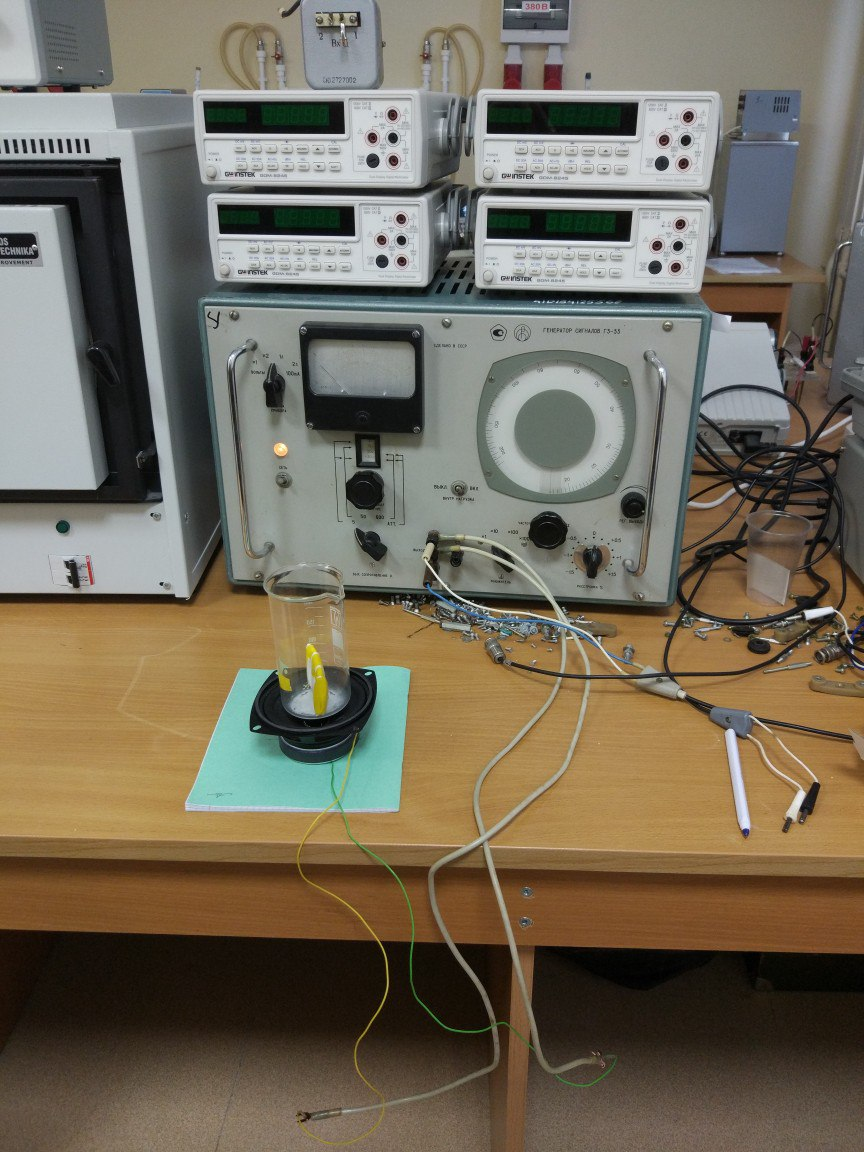
\includegraphics[height=8cm]{img/scheme.jpg}
		\end{minipage}
		\qquad
		\begin{minipage}{0.45 \linewidth}
			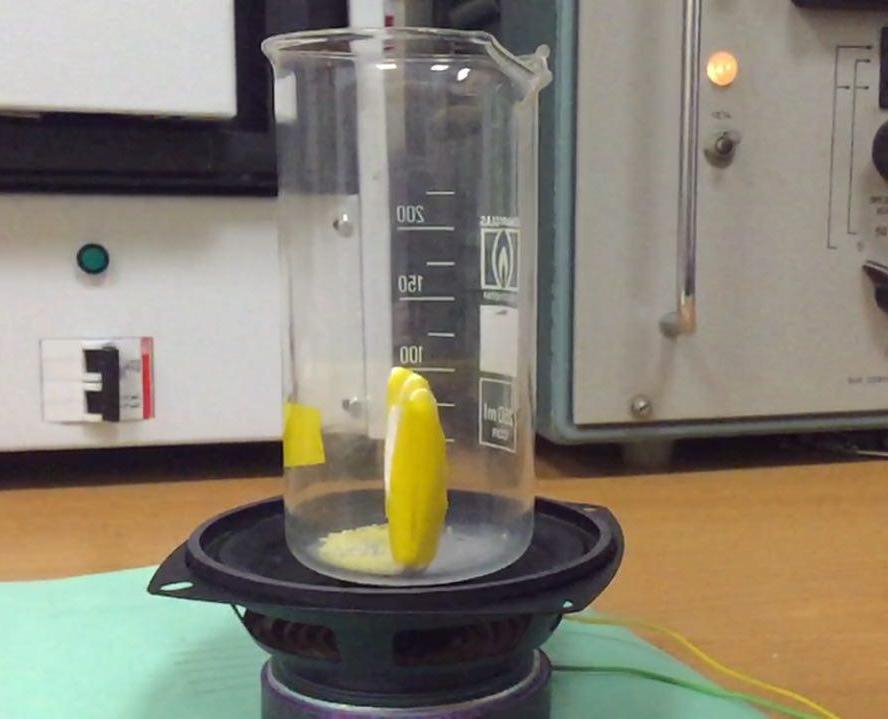
\includegraphics[height=7cm]{img/zoom_scheme.jpg}
		\end{minipage}
	\end{center}
	\caption{Cхема установки}
\end{figure}

В нашем случае возбуждение соответсвует кинетической энергии частиц, приводимых в движение мембраной динамика. Эта энергия пропорциональна квадрату скорости колебаний динамика: $v^2 = f^2 \cdot A^2$. Макроскопическое изменение, соответствующее фазовому переходу, ~--- собиранию шариков в одной из половин цилиндра, разделенных небольшой стенкой. Коэффициент  $\left\lvert \frac{N_1 - N_2}{N_1 + N_2} \right\rvert$ хорошо подходит для параметра порядка.

\emph{Цель работы}: найти зависимость параметра порядка $\eta = \left\lvert \frac{N_1 - N_2}{N_1 + N_2} \right\rvert$ от $| A^2 - A_{cr}^2|$.


\subsubsection*{Ход работы}

\begin{enumerate}
	\item Определение критической амплитуды фазового перехода
	\item Калибровка установки
	\item Определение показателя степени
\end{enumerate}

\emph{Определение критической амплитуды}

Подсоединим динамик к генератору с соблюдением полярности, затем насыпем 60 шариков кускуса в одну из половин цилиндра. Постепенно увеличивая амплитуду, будем записывать выходное напряжение генератора и количество шариков $N_1$ и $N_2$ в каждой половине сосуда.

\begin{figure}
	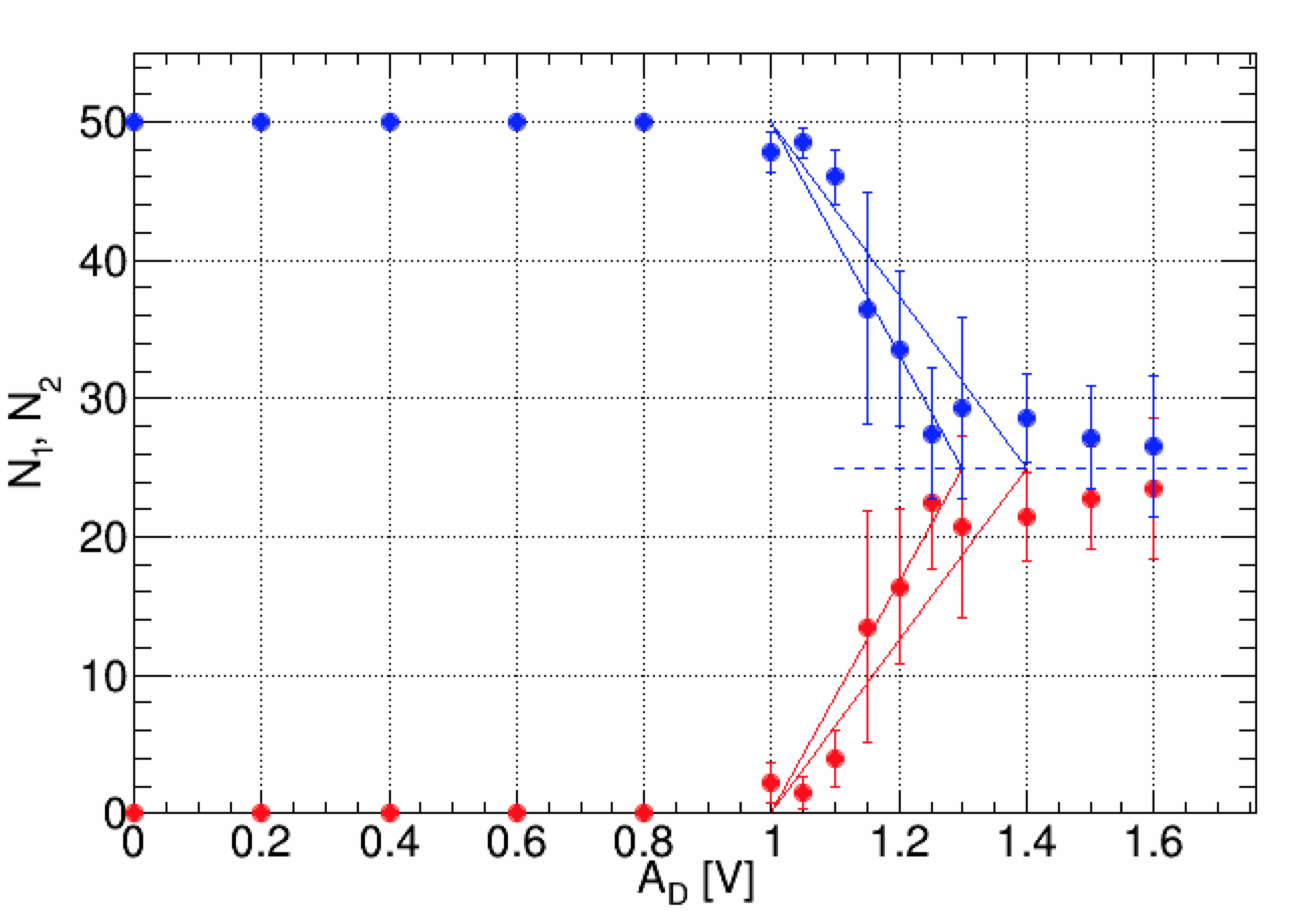
\includegraphics[scale=0.5]{img/N(A).jpg}
	\caption{зависимость $N_1$ и $N_2$ от амплитуды}
\end{figure}

\emph{Калибровка установки}

С помощью замедленной съемки на камере мобильного телефона iPhone 6 и миллиметровой бумаги найдём зависимость реальной амплитуды колебаний мембраны динамика от подаваемого вольтажа.

\begin{figure}
	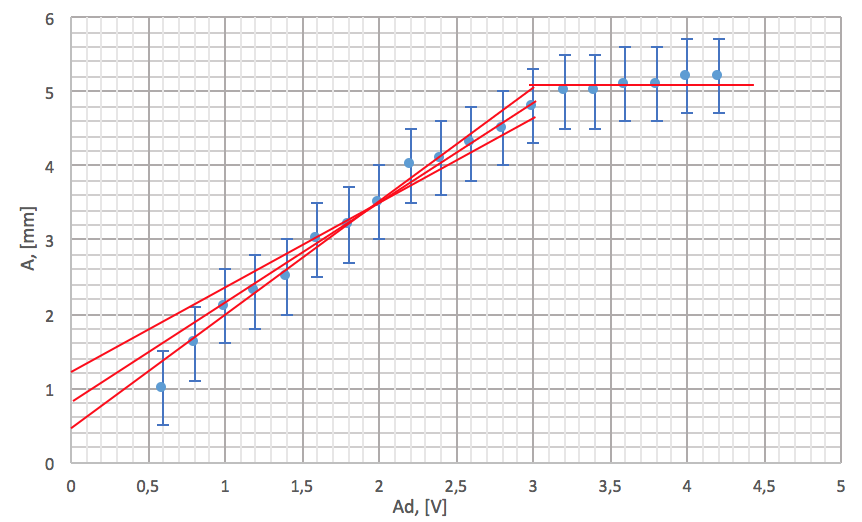
\includegraphics[scale=0.5]{img/A(V).jpg}
	\caption{зависимость амплитуды мембраны от напряжения}
\end{figure}

\emph{Определение показателя степени}

Построим график зависимости $\eta$ от $|A^2 - A_{cr}^2|$:

\begin{figure}[h]
	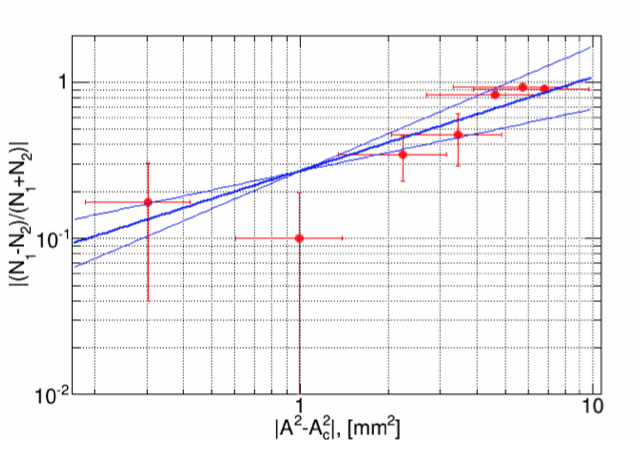
\includegraphics[scale=1]{img/result.jpg}
	\caption{$\eta$ от $|A^2 - A_{cr}^2|$}
\end{figure}

Из графика найдём, что $\eta \sim |A^2 - A_{cr}^2|^{0.6}$, то есть степень $b = 0.6 \pm 0.2$, что хорошо согласуется с предсказываемой теоретической зависимостью $b_{th} = 0.5$.


\subsection*{Вывод}
 
В данной работе была рассмотрена классическая теория фазовых переходов второго рода разработанная Л. Д. Ландау. Полученная физическая модель описывает широкий класс фазовых переходов:  парамагнетик-ферромагнетик или парамагнетик-антиферромагнетик, переходы в сегнетоэлектриках и некоторые другие.

Также была предложена наглядная механическая аналогия модели переходов второго рода. Результаты эксперимента согласуются с физической моделью в пределах погрешности.


\subsection*{Источники}

[1] \textit{Д.\,В. Сивухин.} Общий курс физики. Термодинамика и молекулярная физика.

\vspace{-.7\parskip}
[2] \textit{Л.\,Д. Ландау, Е.\, М. Лифшиц} Том VIII. Электродинамика сплошных сред.

\vspace{-.7\parskip}
[3] \textit{Л.\,Д. Ландау, Е.\, М. Лифшиц} Том V. Статистическая физика.

\end{document}